\documentclass[10pt,a4paper]{report}
\usepackage[latin1]{inputenc}
\usepackage[utf8]{inputenc}
\usepackage{amsmath}
\usepackage{amsfonts}
\usepackage{amssymb}
\usepackage{graphicx}
\usepackage{multicol}
\usepackage{tabularx}
\usepackage{tikz}
\documentclass{standalone}
\documentclass{article}
\usetikzlibrary{arrows,shapes,automata,petri,positioning,calc}

\usepackage{hyperref}
\usepackage{tikz}
\usetikzlibrary{matrix,calc}
\usepackage[margin=0.5in]{geometry}
\newenvironment{Figure}
  {\par\medskip\noindent\minipage{\linewidth}}
  {\endminipage\par\medskip}
\begin{document}
%%%%%%%%%%%%%%%%%-logo figure-%%%%%%%%%%%%%%%%%%%%%%%
\begin{figure*}[!tbp]
  \centering
  \begin{minipage}[b]{0.4\textwidth}
    
\includegraphics[scale = 0.05]{iitlogo.jpg}
  \end{minipage}
  \hfill
  \vspace{5mm}\begin{minipage}[b]{0.4\textwidth}
\raggedleft  
\includegraphics[scale = 0.10]{nrc.png}\

  \end{minipage}\vspace{0.2cm}
\end{figure*}
%--------------------name & rollno-----------------------
\raggedright \textbf{Name}:\hspace{1mm} Chirag Shah\hspace{3cm} \Large \textbf{ASSIGNMENT-1}\hspace{2.5cm} % 
\normalsize \textbf{Roll No.} :\hspace{1mm} FWC22053\vspace{1cm}
\begin{multicols}{2}

\begin{document}
%-----------------Sequence Detector-----------------------------%
\textbf{Sequence Detector}
\vspace{0.5cm}\raggedright \\A sequence detector is a sequential state machine that takes an input string of bits and generates an output 1 whenever the target sequence has been detected. In a Mealy machine, output depends on the present state and the external input (x).\vspace{3mm} \\ 
%------------------------working-------------------%
\textbf{Working}\vspace{1mm}
\raggedright \\A sequence detector accepts as input a string of bits: either 0 or 1. Its output goes to 1 when a target sequence has been detected.\vspace{3mm} \\ 
\raggedright \\There are two basic types:\vspace{3mm} \\
\begin{itemize}
\item Overlap
\item Non-overlap. \vspace{2mm}
\end{itemize}
%----------------problem statement--------------%
\raggedright \textbf{Problem Statement:}\vspace{2mm}
\raggedright \\Using Platformio CLI wite a programm to identify if the Sequence is either  11 or 00110 .

\vspace{5mm}

%-----------------------------solution---------------------------
\raggedright \textbf{SOLUTION}:\vspace{2mm}
\raggedright Steps for using State Diagram:
\\1.To detect 00110 and 11 . first input is given to SO . if the first bit i/p is 0 it will go to next state i.e S1 and o/p will be 0 (LED=OFF) . 
\\2.If the i/p is 1 it will go to state S5. o/p will be 0 (LED=OFF)
\\3.Same steps will be repeated for all states  .
\\4.when it detects 00110 the o/p will be 1 (LED=ON)
\\5.Same as above if it detects 11 o/p will be 1 (LED=ON)
\\6.Again it repeats as it is overlapping. \\

%--------------------state diagram------------------------------%

\vspace{1cm}
\textbf{State Diagram}
\vspace{0.4cm}
\usetikzlibrary{arrows,shapes,automata,petri,positioning,calc}

\tikzset{
    place/.style={
        circle,
        thick,
        draw=black,
        fill=gray!50,
        minimum size=6mm,
    },
        state/.style={
        circle,
        thick,
        draw=blue!75,
        fill=blue!20,
        minimum size=6mm,
    },
}

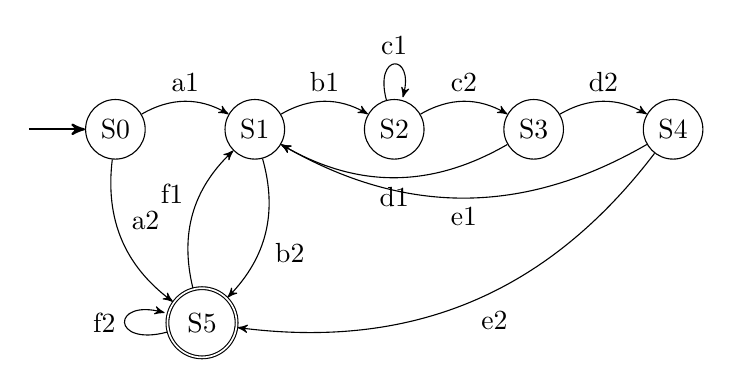
\begin{tikzpicture}[node distance=2cm and 1cm,>=stealth',auto, every place/.style={draw}]
    \node [place] (S0) {S0};
    \coordinate[node distance=1.1cm,left of=S0] (left-S0);
    \coordinate[node distance=1.1cm,right of=S0] (right-S0);

    \draw[->, thick] (left-S0) -- (S0);

    \node [place] (S1) [right=of S0] {S1};
    \node [place] (S2) [right=of S1] {S2};
    \node [place] (S3) [right=of S2] {S3};
    \node [place] (S4) [right=of S3] {S4};
    \node [state,initial text=,accepting by double] (S5) [below =of right-S0] {S5};

    


    \path[->] (S0) edge [bend left] node {a1}(S1);
    \path[->] (S0) edge [bend right] node {a2} (S5);
    
    \path[->] (S1) edge [bend left] node {b1} (S2);
    \path[->] (S1) edge [bend left] node {b2} (S5);
    
    \path[->] (S2) edge [loop above] node {c1} (S2);
    \path[->] (S2) edge [bend left] node {c2} (S3);
    
    \path[->] (S3) edge [bend left] node {d1} (S1);  
    \path[->] (S3) edge [bend left] node {d2} (S4);  
    
    \path[->] (S4) edge [bend left] node {e1} (S1);  
    \path[->] (S4) edge [bend left] node {e2} (S5);  
    
    \path[->] (S5) edge [bend left] node {f1} (S1);  
    \path[->] (S5) edge [loop left] node {f2} (S5);  

\end{tikzpicture}
\vspace{1.5cm}
%-------------------State Diagrams-------------%

\textbf{State Diagram -Input and Outputs}

  \setlength{\arrayrulewidth}{0.5mm} \begin{center}
      

  \setlength{\tabcolsep}{25pt}
  \renewcommand{\arraystretch}{1.3}
  \begin{tabular}{|l|c|c|}
  \hline 
  \textbf{States} & \textbf{Input} & \textbf{output} \\
  \hline
    a1 & 0 & 0\\
    a2 & 1 & 0\\
    b1 & 0 & 0\\
    b2 & 1 & 0\\
    c1 & 0 & 0\\
    c2 & 1 & 0\\
    d1 & 0 & 0\\
    d2 & 1 & 0\\
    e1 & 0 & 1\\
    e2 & 1 & 0\\
    f1 & 0 & 0\\
    f2 & 1 & 1\\
    \hline
      \end{tabular}
  \end{center} \vspace{2mm}
  
  \textbf{Truth table}
  \begin{center}
    \label{tab:truthtable}
    \setlength{\arrayrulewidth}{0.5mm}
\setlength{\tabcolsep}{10pt}
\renewcommand{\arraystretch}{1.5}
    \begin{tabular}{|l|c|r|l|c|l|c|l|}
    \hline % <-- Alignments: 1st column left, 2nd middle and 3rd right, with vertical lines in between
      \textbf{q2} & \textbf{q1} & \textbf{q0} & \textbf{x} & \textbf{d2} & \textbf{d1} & \textbf{d0} & \textbf{y}\\
      \hline  \hline
      0 & 0 & 0 & 0 & 0 & 0 & 1 & 0\\  \hline
      0 & 0 & 0 & 1 & 1 & 0 & 1 & 0\\  \hline
      0 & 0 & 1 & 0 & 0 & 1 & 0 & 0\\  \hline
      0 & 0 & 1 & 1 & 1 & 0 & 1 & 0\\ \hline
      0 & 1 & 0 & 0 & 0 & 1 & 0 & 0\\ \hline
      0 & 1 & 0 & 1 & 0 & 1 & 1 & 0\\  \hline
      0 & 1 & 1 & 0 & 0 & 0 & 1 & 0\\ \hline
      0 & 1 & 1 & 1 & 1 & 0 & 0 & 0\\ \hline
      1 & 0 & 0 & 0 & 0 & 0 & 1 & 1\\ \hline
      1 & 0 & 0 & 1 & 1 & 0 & 1 & 0\\ \hline
      1 & 0 & 1 & 0 & 0 & 0 & 1 & 0\\ \hline
      1 & 0 & 1 & 1 & 1 & 0 & 1 & 1\\ \hline
      1 & 1 & 0 & 0 & x & x & x & x\\ \hline
      1 & 1 & 0 & 1 & x & x & x & x\\ \hline
      1 & 1 & 1 & 0 & x & x & x & x\\ \hline
      1 & 1 & 1 & 1 & x & x & x & x\\ \hline
      1 & 1 & 1 & 1 & x & x & x & x\\ 
      \hline
    \end{tabular}
  \end{center}
 
  %-----boolean expression----%
 \section*{\large Boolean expressions}
The boolean expressions for \textbf{d} and \textbf{x} are:\\
\vspace{2mm}
With don't care(X):\\\vspace{1mm}
\raggedright %Left aligned equations 
&d_2 = q_1'x + q_0x \\ \vspace{1mm}
&d_1 = q1q_0' + q_2'q_1'q0x'\\\vspace{1mm}
&d_0 = q_2 + q_1'q_0' + q_1'x + q_0'x + q_1q_0x'\\\vspace{1mm}
&x = q_2q_0'x' + q_2q_0x \\ \vspace{2mm}

Without don't care(X):\\\vspace{1mm}
\raggedright %Left aligned equations 
&d_2 = q_1'x + q_2'q_0x \\ \vspace{1mm}
&d_1 = q_2'q_1q_0'+q_2'q_1'q_0x'\\\vspace{1mm}
&d_0 = q_1'q_0'+ q_1'x + q_2q_1' + q_2'q_0'x + q_2'q_1q_0x'\\\vspace{1mm}
&x = q_2q_1'q_0'x' + q_2q_1'q_0x \\ \vspace{2mm}
 
 \vspace{2mm} The above truth table can be verified in arduino.\\1.consider 4 digital pins 6,7,8,9 as inputs D9 is given to +vcc or ground. \\2.Consider 4 digital pins 2,3,4,5 as Outputs. Here D5 is given to LED  .\\3. D13 acts as clock signal. \\4. The connections are given in the Hardware Connection table. \\
\vspace{0.5cm}
\textbf{Components}
 \begin{center} \setlength{\arrayrulewidth}{0.5mm} 
  \setlength{\tabcolsep}{18pt}
  \renewcommand{\arraystretch}{1.5}
  \begin{tabular}{|l|c|c|}
  \hline 
  \textbf{Component} & \textbf{Value} & \textbf{Quantity} \\
  \hline \hline
    Breadboard & - & 1\\ \hline
    Resistor & 220 ohms & 1\\ \hline
    Arduino & Uno & 1\\ \hline
    Led & 5v & 1\\ \hline
    Flip Flop & 7474 & 2\\ \hline
    Jumper Wires & - & 20\\ 
   
    \hline
      \end{tabular}
  \end{center}
  %--------------IC diagram--------%
   \vspace{2mm}\textbf{7474 IC Pin details}
 \begin{center}
 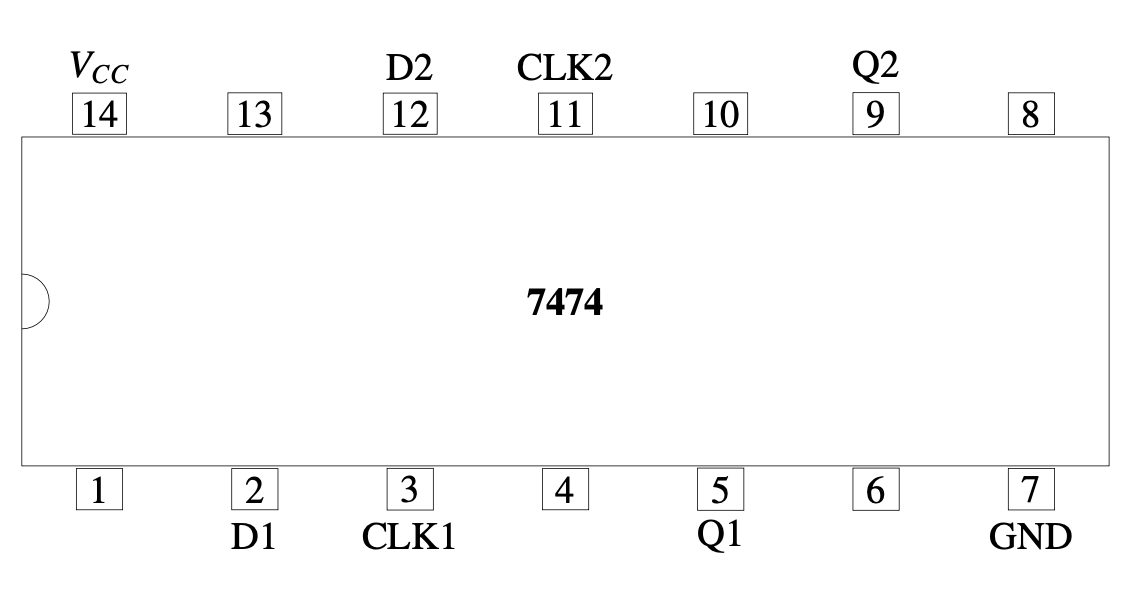
\includegraphics[width=0.45\textwidth]{ic.png} 
 \end{center}
 %----------DFF--------%
  \vspace{2mm}\textbf{D Flip-Flop}
 \begin{center}
 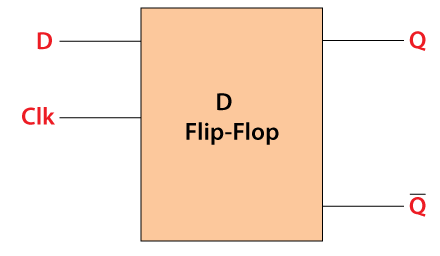
\includegraphics[width=0.45\textwidth]{dff.jpg} 
 \end{center}
 \textbf{Working of D Flip-Flop}

  \setlength{\arrayrulewidth}{0.5mm} \begin{center}
      

  \setlength{\tabcolsep}{25pt}
  \renewcommand{\arraystretch}{1.3}
  \begin{tabular}{|l|c|l|c|}
  \hline 
  \textbf{CLK} & \textbf{D} & \textbf{Q}  & \textbf{$\overline{\textbf{Q}}$}\\
  \hline
    0 & 0 & Q & $\overline{Q}$\\
    0 & 1 & Q & $\overline{Q}$ \\
    1 & 0 & 0 & 1\\
    1 & 1 & 1 & 0\\
    \hline
      \end{tabular}
  \end{center} \vspace{2mm}
  
The D flip-flop is a clocked flip-flop with a single digital input 'D'. \\ Each time a D flip-flop is clocked, its output follows the state of 'D'.\\
\vspace{1cm}
\textbf{Hardware Connections }
\begin{center}
\setlength{\arrayrulewidth}{0.5mm}
\setlength{\tabcolsep}{0.9pt}
\renewcommand{\arraystretch}{2}
    \begin{tabular}{|l|c|l|c|l|c|l|c|l|c|}
    \hline 
    \textbf{Arduino pins} & \textbf{D6} & \textbf{D7} & \textbf{D8} & \textbf{ D9} & \textbf{D2} & \textbf{D3} & \textbf{D4} & \textbf{D5}& \textbf{D13}\\
    \hline
    7474 (2-FF) & 5 & 9 &  &  & 2 & 12 &  &  & CLK \\  \hline
    7474 (1-FF) &  &  & 5 &  &  &  & 2 &  & CLK \\ \hline
    I/P &  &  &   & 5v/GND &  &  &   &    &   \\ \hline
    Detector&  &  &   &  &  &  &   & LED &  \\ 
    \hline
      \end{tabular}
  \end{center}
  
\raggedright  Download the code from the link below and upload into the arduino\\
Github link: \href{https://github.com/chiragshah1244/FWC-/blob/main/assignments/assignment-1/src/seq.cpp}{Assignment-1}.

  \end{multicols}
\end{document}